\documentclass[11pt]{article}
\usepackage{amsmath, amssymb, amsthm, enumitem, hyperref}
\usepackage{pdfpages}

% Page formatting
\usepackage[margin=1in]{geometry}
\setlength{\parskip}{0.5em}
\setlength{\parindent}{0em}

% Theorem environments
\newtheorem{theorem}{Theorem}[section]
\newtheorem{lemma}[theorem]{Lemma}
\newtheorem{corollary}[theorem]{Corollary}
\newtheorem{proposition}[theorem]{Proposition}

\theoremstyle{definition}
\newtheorem{definition}[theorem]{Definition}
\newtheorem{example}[theorem]{Example}
\newtheorem{exercise}[theorem]{Exercise}

\theoremstyle{remark}
\newtheorem{remark}[theorem]{Remark}

% Custom commands
\newcommand{\R}{\mathbb{R}}
\newcommand{\N}{\mathbb{N}}
\newcommand{\Z}{\mathbb{Z}}


\title{Math 51 Notes}
\author{Sreeprasad Govindankutty}
\date{\today}

\begin{document}

\maketitle
\tableofcontents
\newpage

% Chapter 1
\section{Planes in \mathbb{R}^3}

\subsection{Exercise 3.1}
Consider the three different points $(3,-2,5)$, $(\frac{1}{2},0,4)$, and $(1,-2,10)$ in $\mathbb{R}^3$.

(a) Use difference vectors to show these points are not on a common line, so there is exactly one plane $\mathcal{P}$ containing all of them.
Let 
\[
P = (3,-2,5)
\]
\[
Q = \frac{1}{2},0,4
\]
\[
R = (1,-2,10)
\]

\[
\overrightarrow{PQ} = Q - P = \begin{bmatrix}
\frac{5}{2} \\ 2 \\ -1
\end{bmatrix}
\]

\[
\overrightarrow{PR} = R - P = \begin{bmatrix}
-2 \\ 0 \\ 5
\end{bmatrix}
\]

we need to check whether $\overrightarrow{PQ}$ and $\overrightarrow{PR}$ are linearly independent.
There should not be any scalar a and b both non-zero such that
\[
a \overrightarrow{PQ} + b \overrightarrow{PR} = 0
\]

\[
a . \begin{bmatrix}
\frac{5}{2} \\ 2 \\ -1
\end{bmatrix} + b . \begin{bmatrix}
-2 \\ 0 \\ 5
\end{bmatrix} = 0
\]
\[
\frac{5}{2}a - 2b = 0
\]
\[
2a  = 0
\]
\[
-a + 5b = 0
\]
Substituting
\[
a = 0
\]
we get
\[
 0 + 5.b =0
\]
This gives
\[
a = 0, b = 0
\]
This shows that $\overrightarrow{PQ}$ and $\overrightarrow{PR}$ are linearly independent.


(b) Give a parametric form for the plane $\mathcal{P}$ from (a).

The plane consists of all vectors of the form
\[
P + t\overrightarrow{PQ}+t^\prime\overrightarrow{PR} 
\]
for scalars t and t'
\[
\begin{bmatrix}
3 \\ -2 \\ 5
\end{bmatrix} + t \begin{bmatrix}
\frac{5}{2} \\ 2 \\ -1
\end{bmatrix} + t^\prime \begin{bmatrix}
-2 \\ 0 \\ 5
\end{bmatrix}
\]
The parametric form of equation is
\[
X =
\begin{bmatrix}
    3+\frac{5}{2} t -2 t^\prime \\ 
    -2 + 2t  \\
    5 - t + 5 t^\prime \\
\end{bmatrix}
\]
\subsection{Exercise 3.2}
Give an equation describing the plane $\mathcal{P}$ in Exercise 3.1

Let non-zero vector n = 
\[
\begin{bmatrix}
a \\ b \\ c
\end{bmatrix}
\]
that is perpendicular to all direction of plane in Exercise 3.1

As the normal vector n is perpendicular we have 
\[
n . \overrightarrow{PQ} = 0 
\]
\[
n . \overrightarrow{PR} = 0
\]

\[
\begin{bmatrix}
a \\ b \\ c 
\end{bmatrix} . 
\begin{bmatrix}
\frac{5}{2} \\ 2 \\ -1
\end{bmatrix}
 = 0
\]
\[
\begin{bmatrix}
a \\ b \\ c 
\end{bmatrix} . 
\begin{bmatrix}
-2 \\ 0 \\ 5
\end{bmatrix}
 = 0
\]
\[
\frac{5}{2} a + 2b - c = 0
\]
\[
-2a + 5c = 0
\]
Substituting c = $\frac{5}{2}$a + 2b
we get 
\[
-2a + 5(\frac{5}{2}a + 2b) =0
\]
\[
-4a + 25a + 20b= 0
\]
\[
\frac{-21}{20}a =  b
\]
\[
c = \frac{5}{2}a +2*\frac{-21}{20}a
\]
\[
c = \frac{9}{20}a
\]
It follows that n = 
\[
\begin{bmatrix}
a \\ \frac{-21}{20}a \\ \frac{9}{20}a
\end{bmatrix}
\]
when n $\neq$ 0  and  a $\neq$ 0, let's put a = 1
\[
\begin{bmatrix}
1 \\ \frac{-21}{20} \\ \frac{9}{20}
\end{bmatrix}
\]
Finally let 
\[
\begin{bmatrix}
x \\ y \\ z
\end{bmatrix}
\]
be a point on the plane. The vector from P (3,-2,5) to the above point is 
the difference vector 
\[
\begin{bmatrix}
    x - 3 \\ y -2 \\ z - 5
\end{bmatrix}
\]
The vector from P (3,-2,5) to the above point is perpendicular to the normal vector n,
So
\[
\begin{bmatrix}
    x - 3 \\ y -2 \\ z - 5
\end{bmatrix} . \begin{bmatrix}
1 \\ \frac{-21}{20} \\ \frac{9}{20}
\end{bmatrix} = 0 
\]
\[
x - 3 - (y-3)\frac{21}{20} +(z-5).\frac{9}{20}=0
\]
\[
20x - 60 - 21y + 63 + 9z - 45 = 0 
\]
\[
20x-21y+9z =42
\]
\subsection{Exercise 3.3}
Find the parametric form for the plane $\mathbb{R}^3$ given by the equation 
\[
6x-6y-z=7
\]
\subsection{Exercise 3.4}
Find the equation for the plane parallel to 
\[
4x-7y+2z=1
\]
and passing through the point
\[
\begin{bmatrix}
1 \\ 2 \\ 3.
\end{bmatrix}
\]



\section{Span, subspaces, and dimension}

\subsection{Exercise 4.1}

\begin{enumerate}
    \item[(a)] \[
\left\{
\begin{bmatrix}
x \\ y \\ z
\end{bmatrix}
\in \mathbb{R}^3 : z = 2x - y
\right\}
\]

A set of vectors \( S \subseteq \mathbb{R}^n \) is a linear subspace if and only if:
\begin{enumerate}
    \item The zero vector is in \( S \).
    \item \( S \) is closed under vector addition: if \( \mathbf{u}, \mathbf{v} \in S \), then \( \mathbf{u} + \mathbf{v} \in S \).
    \item \( S \) is closed under scalar multiplication: if \( \mathbf{u} \in S \) and \( c \in \mathbb{R} \), then \( c \cdot \mathbf{u} \in S \).
\end{enumerate}

Checking each condition:
\begin{enumerate}
    \item \textbf{The zero vector is in \( S \).}
    \[
    \mathbf{u} = 
    \begin{bmatrix} 
    0 \\ 0 \\ 0
    \end{bmatrix}
    \]
    Check if it satisfies \( z = 2x - y \): 
    \[
    2 \cdot 0 - 0 = 0.
    \]
    This is true, so the zero vector is in the set.

    \item \textbf{\( S \) is closed under vector addition.}

    Let 
    \[
    \mathbf{u} = 
    \begin{bmatrix} 
    x_1 \\ y_1 \\ z_1
    \end{bmatrix}, \quad 
    \mathbf{v} = 
    \begin{bmatrix} 
    x_2 \\ y_2 \\ z_2
    \end{bmatrix}.
    \]

    \[
    \mathbf{u} + \mathbf{v} = 
    \begin{bmatrix} 
    x_1 + x_2 \\ y_1 + y_2 \\ z_1 + z_2
    \end{bmatrix}.
    \]

    \[
    z_1 + z_2 = 2 \cdot (x_1 + x_2) - (y_1 + y_2).
    \]

    \[
    z_1 = 2 \cdot x_1 - y_1, \quad z_2 = 2 \cdot x_2 - y_2.
    \]

    \[
    z_1 + z_2 = 2 \cdot (x_1 + x_2) - (y_1 + y_2).
    \]
    Thus, the set is closed under addition.

    \item \textbf{\( S \) is closed under scalar multiplication.}

    Let
    \[
    \mathbf{u} = 
    \begin{bmatrix} 
    x  \\ y \\ z
    \end{bmatrix}.
    \]
    \[
    c \cdot \mathbf{u} = 
    \begin{bmatrix} 
    cx  \\ cy \\ cz
    \end{bmatrix}.
    \]

    \[
    cz = 2 \cdot (cx) - (cy).
    \]
    But 
    \[
    z = 2x - y.
    \]
    So 
    \[
    cz = c (2x-y) = 2 \cdot (cx) - (cy).
    \]
    Thus, the set is closed under scalar multiplication. So this is a linear subspace.
\end{enumerate}

    \item[(b)] \[
\left\{
\begin{bmatrix}
x \\ y \\ z
\end{bmatrix}
\in \mathbb{R}^3 : z = 1 + 2x - y
\right\}
\]

A set of vectors \( S \subseteq \mathbb{R}^n \) is a linear subspace if and only if:
\begin{enumerate}
    \item The zero vector is in \( S \).
    \item \( S \) is closed under vector addition: if \( \mathbf{u}, \mathbf{v} \in S \), then \( \mathbf{u} + \mathbf{v} \in S \).
    \item \( S \) is closed under scalar multiplication: if \( \mathbf{u} \in S \) and \( c \in \mathbb{R} \), then \( c \cdot \mathbf{u} \in S \).
\end{enumerate}


Checking each condition:
\begin{enumerate}
    \item \textbf{The zero vector is in \( S \).}
    \[
    \mathbf{u} = 
    \begin{bmatrix} 
    0 \\ 0 \\ 0
    \end{bmatrix}
    \]
    Check if it satisfies \( z = 1 + 2x - y \): 
    \[
    2 \cdot 0 - 0 = 1 \neq 0
    \]

This is false, so the zero vector is not in the set.
So this is not a linear subspace.
\end{enumerate}
    \item[(c)] \[
\left\{
\begin{bmatrix}
x \\ y
\end{bmatrix}
\in \mathbb{R}^2 : y = x^2
\right\}
    \]
A set of vectors \( S \subseteq \mathbb{R}^n \) is a linear subspace if and only if:
\begin{enumerate}
    \item The zero vector is in \( S \).
    \item \( S \) is closed under vector addition: if \( \mathbf{u}, \mathbf{v} \in S \), then \( \mathbf{u} + \mathbf{v} \in S \).
    \item \( S \) is closed under scalar multiplication: if \( \mathbf{u} \in S \) and \( c \in \mathbb{R} \), then \( c \cdot \mathbf{u} \in S \).
\end{enumerate}


Checking each condition:
\begin{enumerate}
    \item \textbf{The zero vector is in \( S \).}
    \[
    \mathbf{u} = 
    \begin{bmatrix} 
    0 \\ 0 
    \end{bmatrix}
    \]
    Check if it satisfies \( y = x^2 \): 
    \[
    0 = 0^2 = 0
    \]

This is true, so the zero vector is in the set.
 \item \( S \) is closed under vector addition: if \( \mathbf{u}, \mathbf{v} \in S \), then \( \mathbf{u} + \mathbf{v} \in S \).


 Let 
    \[
    \mathbf{u} = 
    \begin{bmatrix} 
    x_1 \\ y_1
    \end{bmatrix}, \quad 
    \mathbf{v} = 
    \begin{bmatrix} 
    x_2 \\ y_2
    \end{bmatrix}.
    \]

    \[
    \mathbf{u} + \mathbf{v} = 
    \begin{bmatrix} 
    x_1 + x_2 \\ y_1 + y_2
    \end{bmatrix}.
    \]

    \[
    y_1 + y_2 = (x_1 + x_2)^2
    \]
    Here
    \[
    y1 = x1^2, y2 = x2^2
    \]
    \[
    y1+y2 = x1^2 + x2^2 \neq (x1+x2)^2
    \]
\( S \) is NOT closed under vector addition. So this is not a linear subspace.
    
\end{enumerate}
    \item[(d)] \[
    \left\{
    \begin{bmatrix}
    x \\ y \\ z
    \end{bmatrix}
    \in \mathbb{R}^3 : 
    \begin{aligned}
    3x - y + z &= 0, \\
    x + y - 4z &= 0
    \end{aligned}
    \right\}
\]
A set of vectors \( S \subseteq \mathbb{R}^n \) is a linear subspace if and only if:
\begin{enumerate}
    \item The zero vector is in \( S \).
    \item \( S \) is closed under vector addition: if \( \mathbf{u}, \mathbf{v} \in S \), then \( \mathbf{u} + \mathbf{v} \in S \).
    \item \( S \) is closed under scalar multiplication: if \( \mathbf{u} \in S \) and \( c \in \mathbb{R} \), then \( c \cdot \mathbf{u} \in S \).
\end{enumerate}


Checking each condition:
\begin{enumerate}
    \item \textbf{The zero vector is in \( S \).}
    \[
    \mathbf{u} = 
    \begin{bmatrix} 
    0 \\ 0 \\ 0
    \end{bmatrix}
    \]
    Check if it satisfies 
    \[
     \begin{aligned}
    3x - y + z &= 0, \\
    x + y - 4z &= 0
    \end{aligned}
    \]
     \[
    3 \cdot 0 - 0 + 0 = 0
    \]
     \[
    0 + 0 - 4.0 = 0
    \]
    This is true, so the zero vector is in the set.
  \item 
   \item \textbf{\( S \) is closed under vector addition.}

    Let 
    \[
    \mathbf{u} = 
    \begin{bmatrix} 
    x_1 \\ y_1 \\ z_1
    \end{bmatrix}, \quad 
    \mathbf{v} = 
    \begin{bmatrix} 
    x_2 \\ y_2 \\ z_2
    \end{bmatrix}.
    \]

    \[
    \mathbf{u} + \mathbf{v} = 
    \begin{bmatrix} 
    x_1 + x_2 \\ y_1 + y_2 \\ z_1 + z_2
    \end{bmatrix}.
    \]
    \[
     \begin{aligned}
    3x - y + z &= 0, \\
    x + y - 4z &= 0
    \end{aligned}
    \]
    
    \[
     z = -3x + y \]
    \[
     z = (x+y)/4
    \]
    
    \[
    z_1 + z_2 = -3(x_1+x_2) +y
    \]
    \[
    -3(x_1)+y_1 + -3(x_2)+y_2 = -3(x_1+x_2) +y_1+y_2
    \]
    \[
    -3(x_1+x_2)+y_1+y_2 = -3(x_1+x_2) +y_1+y_2
    \]
    
    \[
    z1 + z_2 = (x_1+x_2+y_1+y_2)/4
    \]
    \[
    (x_1+y_1)/4 + (x_2+y_2)/4 = (x_1+x_2+y_1+y_2)/4
    \]
    \[
    (x_1+y_1 + x_2+y_2)/4 = (x_1+x_2+y_1+y_2)/4
    \]
    This is true so \( S \) is closed under vector addition.
    \item \textbf{\( S \) is closed under scalar multiplication.}

    Let
    \[
    \mathbf{u} = 
    \begin{bmatrix} 
    x  \\ y \\ z
    \end{bmatrix}.
    \]
    \[
    c \cdot \mathbf{u} = 
    \begin{bmatrix} 
    cx  \\ cy \\ cz
    \end{bmatrix}.
    \]
    \[
    cz = -3cx_1+cy_1
    \]
     \[
    c(-3x_1+y_1) = -3cx_1+cy_1
    \]
     \[
    -3cx_1+cy_1 = -3cx_1+cy_1
    \]

    \[
    cz_1 = (cx_1 +cy_1)/4
    \]

     \[
    c(x_1+y_1)/4 = (cx_1 +cy_1)/4
    \]
     \[
     (cx_1+cy_1)/4 = (cx_1 +cy_1)/4
    \]
     This is true so \( S \) is closed under scalar multiplication.
     So this is a linear subspace.
\end{enumerate}
\end{enumerate}

\subsection{Exercise 4.2}
For 
\[
v = 
\begin{bmatrix}
2 \\
0 \\
1
\end{bmatrix}
\quad \text{and} \quad
w = 
\begin{bmatrix}
-1 \\
1 \\
3
\end{bmatrix},
\]
find scalars $a$, $b$, $c$ so that
\[
\text{span}(v, w) = \left\{
\begin{bmatrix}
x \\
y \\
z
\end{bmatrix} \in \mathbb{R}^3 : ax + by + cz = 0
\right\}.
\]

Here 
ax + by + cz = 0

From \[
v = 
\begin{bmatrix}
2 \\
0 \\
1
\end{bmatrix}
\]
we have 
\[
a(2) + 0(b) + 1(c) = 0
\]
\[
c = -2(a)
\]

From \[
w = 
\begin{bmatrix}
-1 \\
1 \\
3
\end{bmatrix}
\]
we have 
\[
a(-1) + 1(b) + 3(c) = 0
\]
\[
b = a-3c
\]
Therefore we have scalars a,b,c such that 
\[
 b= a-3c
 \]
\[ c = -2a
\]
Substituting a =1
\[
c=-2
\]
\[
b = 1-3(-2.1) = 7
\]
Substituting we have 
\[
1(x) + 7(y) + -2(z) = 0
\]

From \[
v = 
\begin{bmatrix}
2 \\
0 \\
1
\end{bmatrix}
\]
\[
1(x) + 7(y) + -2(z) = 0
\]
we have 
\[
1(2) + 7(0) + -2(1) = 2 - 2 =0
\]


From \[
w = 
\begin{bmatrix}
-1 \\
1 \\
3
\end{bmatrix}
\]

we have
\[
1(x) + 7(y) + -2(z) = 0
\]
\[
1(-1) + 7(1) + -2(3) 
\]
\[
= -1 + 7 + -6 = -7 + 7 = 0
\]
The resulting triplets work.
\subsection{Exercise 4.3}


For 
\[
v = 
\begin{bmatrix}
1 \\
1 \\
1
\end{bmatrix}
\quad \text{and} \quad
w = 
\begin{bmatrix}
4 \\
2 \\
1
\end{bmatrix},
\]
find scalars $a$, $b$, $c$ so that
\[
\text{span}(v, w) = \left\{
\begin{bmatrix}
x \\
y \\
z
\end{bmatrix} \in \mathbb{R}^3 : ax + by + cz = 0
\right\}.
\]

For 
\[
v = 
\begin{bmatrix}
1 \\
1 \\
1
\end{bmatrix}
\quad \text{and} \quad
w = 
\begin{bmatrix}
4 \\
2 \\
1
\end{bmatrix},
\]
find scalars $a$, $b$, $c$ so that
\[
\text{span}(v, w) = \left\{
\begin{bmatrix}
x \\
y \\
z
\end{bmatrix} \in \mathbb{R}^3 : ax + by + cz = 0
\right\}.
\]

Here 
ax + by + cz = 0

From \[
v = 
\begin{bmatrix}
1 \\
1 \\
1
\end{bmatrix}
\]
we have 
\[
a(1) + 1(b) + 1(c) = 0
\]
\[
b = -(a+c)
\]

From \[
w = 
\begin{bmatrix}
4 \\
2 \\
1
\end{bmatrix}
\]
we have 
\[
a(4) + 2(b) + 1(c) = 0
\]
\[
c = -(4a+2b)
\]
Therefore we have scalars a,b,c such that 
\[
 b= -(a+c)
 \]
\[ c = -(4a+2b)
\]
Substituting a =1 and solving for b and c we get
\[
c=2
\]
\[
b =-3
\]
Substituting we have 
\[
1(x) -3(y) + 2(z) = 0
\]

From \[
v = 
\begin{bmatrix}
1 \\
1 \\
1
\end{bmatrix}
\]
\[
1(x)-3(y) + 2(z) = 0
\]
we have 
\[
1(1) -3(1) + 2(1) = 3 - 3 =0
\]


From \[
w = 
\begin{bmatrix}
4 \\
2 \\
1
\end{bmatrix}
\]

we have
\[
1(x) -3(y) + 2(z) = 0
\]
\[
1(4) + -3(2) + 2(1)
\]
\[
= 6 - 6 = 0
\]
The resulting triplets work.
\subsection{Exercise 4.4}
For the 4-vectors 
\[
w = 
\begin{bmatrix}
-2 \\
2 \\
1 \\
1
\end{bmatrix}
\quad \text{and} \quad
w' = 
\begin{bmatrix}
3 \\
4 \\
0 \\
1
\end{bmatrix},
\]
show that the collection of vectors
\[
V = \left\{ 
x = 
\begin{bmatrix}
x_1 \\
x_2 \\
x_3 \\
x_4
\end{bmatrix} 
\in \mathbb{R}^4 : x \cdot w = 0, \, x \cdot w' = 0
\right\}
\]
is a linear subspace of $\mathbb{R}^4$ in each of the following ways:

\begin{enumerate}
    \item[(a)] For $x \in V$, solve for each of $x_3$ and $x_4$ in terms of $x_1$ and $x_2$ to write $V$ as a span of two vectors;
    \item[(b)] For $x \in V$, solve for each of $x_1$ and $x_4$ in terms of $x_2$ and $x_3$ to write $V$ as a span of two vectors.
\end{enumerate}

Solution:
\begin{enumerate}


\item[(a)] For \(w\),
\[
w \cdot x = -2x_1 + 2x_2 + x_3 + x_4 = 0 \quad \Rightarrow \quad x_3 + x_4 = 2x_1 - 2x_2 \tag{1}
\]
For \(w'\),
\[
w' \cdot x = 3x_1 + 4x_2 + x_4 = 0 \quad \Rightarrow \quad x_4 = -3x_1 - 4x_2 \tag{2}
\]
Substitute \(x_4\) from (2) into (1):
\[
x_3 + (-3x_1 - 4x_2) = 2x_1 - 2x_2
\]
\[
x_3 = 5x_1 + 2x_2 \tag{3}
\]
Thus, the components of \(x\) are:
\[
x_3 = 5x_1 + 2x_2, \quad x_4 = -3x_1 - 4x_2
\]
Substitute these into \(x\):
\[
x =
\begin{bmatrix}
x_1 \\
x_2 \\
5x_1 + 2x_2 \\
-3x_1 - 4x_2
\end{bmatrix}
= x_1
\begin{bmatrix}
1 \\
0 \\
5 \\
-3
\end{bmatrix}
+ x_2
\begin{bmatrix}
0 \\
1 \\
2 \\
-4
\end{bmatrix}
\]
The basis vectors are:
\[
\begin{bmatrix}
1 \\
0 \\
5 \\
-3
\end{bmatrix}, \quad
\begin{bmatrix}
0 \\
1 \\
2 \\
-4
\end{bmatrix}.
\]

\item[(b)] For \(w\),
\[
w \cdot x = -2x_1 + 2x_2 + x_3 + x_4 = 0 \quad \Rightarrow \quad x_4 = -2x_1 + 2x_2 - x_3 \tag{4}
\]
For \(w'\),
\[
w' \cdot x = 3x_1 + 4x_2 + x_4 = 0 \quad \Rightarrow \quad x_4 = -3x_1 - 4x_2 \tag{5}
\]
Equating \(x_4\) from (4) and (5):
\[
-2x_1 + 2x_2 - x_3 = -3x_1 - 4x_2
\]
Simplify:
\[
x_1 + 6x_2 - x_3 = 0 \quad \Rightarrow \quad x_1 = -6x_2 + x_3 \tag{6}
\]
Substitute \(x_1\) from (6) into (4):
\[
x_4 = -2(-6x_2 + x_3) + 2x_2 - x_3
\]
\[
x_4 = 12x_2 - 2x_3 + 2x_2 - x_3
\]
\[
x_4 = 14x_2 - 3x_3 \tag{7}
\]
Thus, the components of \(x\) are:
\[
x_1 = -6x_2 + x_3, \quad x_4 = 14x_2 - 3x_3
\]
Substitute these into \(x\):
\[
x =
\begin{bmatrix}
-6x_2 + x_3 \\
x_2 \\
x_3 \\
14x_2 - 3x_3
\end{bmatrix}
= x_2
\begin{bmatrix}
-6 \\
1 \\
0 \\
14
\end{bmatrix}
+ x_3
\begin{bmatrix}
1 \\
0 \\
1 \\
-3
\end{bmatrix}
\]
The basis vectors are:
\[
\begin{bmatrix}
-6 \\
1 \\
0 \\
14
\end{bmatrix}, \quad
\begin{bmatrix}
1 \\
0 \\
1 \\
-3
\end{bmatrix}.
\]

\end{enumerate}
\subsection{Exercise 4.5}


Find a nonzero 3-vector \(\mathbf{v}\) so that
\[
\left\{
\mathbf{x} \in \mathbb{R}^3 : \mathbf{x} \cdot 
\begin{bmatrix}
3 \\
2 \\
1
\end{bmatrix} 
= 0, \, 
\mathbf{x} \cdot 
\begin{bmatrix}
-2 \\
-1 \\
1
\end{bmatrix} 
= 0
\right\}
= \text{span}(\mathbf{v}).
\]
Then, using the \textit{geometric} fact that any two different planes through the origin in \(\mathbb{R}^3\) meet along a line through the origin, interpret this algebraic outcome that the left side is the span of a single vector.

Solution:

Let a,b,c be scalar so that 

\[
3a+2b+c=0
\]
\begin{equation}
    b = \frac{-c-3a}{2}
\end{equation}
\[
-2a-b+c=0
\]
\[
-2a- \frac{-c-3a}{2}+c=0
\]
\[
c=\frac{a}{3}
\]
\[
2b=-\frac{a}{3}-3a
\]
\[
b=-\frac{5a}{3}
\]
writing v in terms of a,
\[
\begin{bmatrix}
a \\
-\frac{5a}{3} \\
\frac{a}{3}
\end{bmatrix} 
\]

\[
v =
a .  \begin{bmatrix}
1\\
-\frac{5}{3} \\
\frac{1}{3}
\end{bmatrix} 
\]
The two planes defined by the equations
\begin{equation}
    3a+2b+c=0
\end{equation}
\begin{equation}
    -2a-b+c=0
\end{equation}
intersect along a line through the origin in \(\mathbb{R}^3\)
This line is spanned by the vector v. Hence, the solution set is
\[
a .  \begin{bmatrix}
1\\
-\frac{5}{3} \\
\frac{1}{3}
\end{bmatrix} 
\]
Here a $\neq$ 0
so the span is
\[
\begin{bmatrix}
1\\
-\frac{5}{3} \\
\frac{1}{3}
\end{bmatrix} 
\]
\subsection{Exercise 4.6}
 Find a pair of 3-vectors \(\mathbf{v}, \mathbf{w}\) so that
\[
\left\{
\begin{bmatrix}
x \\
y \\
z
\end{bmatrix}
\in \mathbb{R}^3 : 2x - 3y + 2z = 0
\right\}
= \text{span}(\mathbf{v}, \mathbf{w}).
\]


we have 
\[
 2x - 3y + 2z = 0
\]
 Therefore
\[
 x  = \frac{3y-2z}{2}
\]
we can write x=
\[
\begin{bmatrix}
x \\
y \\
z
\end{bmatrix}
\]
as x=
\[
\begin{bmatrix}
\frac{3y-2z}{2} \\
y \\
z
\end{bmatrix}
\]
x= 
\[
y 
\begin{bmatrix}
\frac{3}{2} \\
1 \\
0
\end{bmatrix}
+ z
\begin{bmatrix}
-1 \\
0 \\
1
\end{bmatrix}
\]
Two linearly independent vectors spanning the subspace are:

\[
v1=
\begin{bmatrix}
\frac{3}{2} \\
1 \\
0
\end{bmatrix}
\]
and
\[
 v2=
\begin{bmatrix}
-1 \\
0 \\
1
\end{bmatrix}
\]
\subsection{Exercise 4.7}
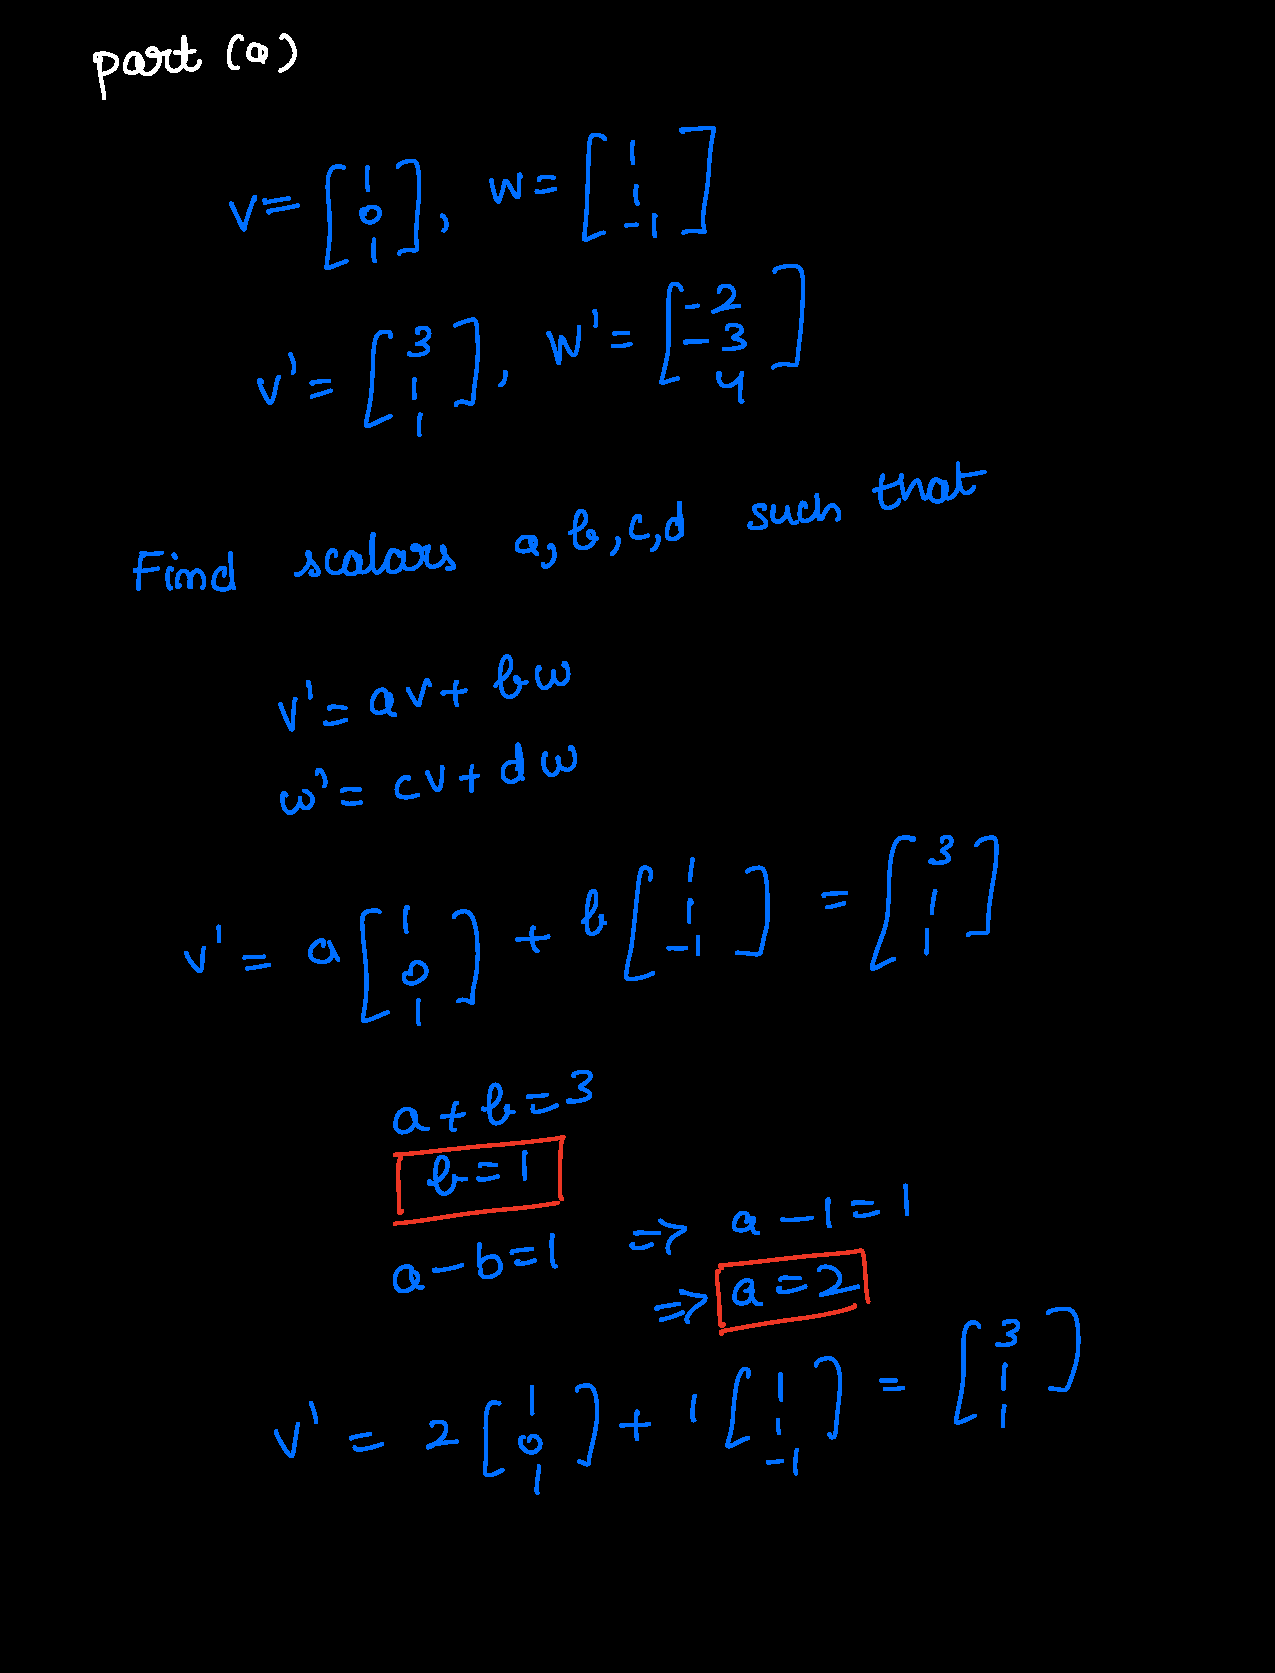
\includepdf[pages=-]{exercises/exercise_4_7.pdf}
\subsection{Exercise 4.8}
Use Theorem 4.2.5 to determine the dimension (1, 2, or 3) of each of the following linear subspaces in $\mathbb{R}^3$. Show the work to justify your answer.

\begin{enumerate}
    \item[(a)] $\text{span}(\mathbf{v}, \mathbf{w})$ for 
    \[
    \mathbf{v} =
    \begin{bmatrix}
    -2 \\ 1 \\ 1
    \end{bmatrix},
    \quad
    \mathbf{w} =
    \begin{bmatrix}
    1 \\ 1 \\ 1
    \end{bmatrix}.
    \]
    \item[(b)] $\text{span}(\mathbf{v'}, \mathbf{w'})$ for 
    \[
    \mathbf{v'} =
    \begin{bmatrix}
    3 \\ 6 \\ -2
    \end{bmatrix},
    \quad
    \mathbf{w'} =
    \begin{bmatrix}
    -2 \\ -4 \\ 2
    \end{bmatrix}.
    \]
    \item[(c)] $\text{span}(\mathbf{v''}, \mathbf{w''},\mathbf{u''})$ for 
    \[
    \mathbf{v''} =
    \begin{bmatrix}
    1 \\ -2 \\ 3
    \end{bmatrix},
    \quad
    \mathbf{w''} =
    \begin{bmatrix}
    4 \\ 0 \\ 2
    \end{bmatrix},
    \quad
    \mathbf{u''} =
    \begin{bmatrix}
    3 \\ -2 \\ 4
    \end{bmatrix}.
    \]
\end{enumerate}

Solution:

\begin{enumerate}
    \item[(a)] $\text{span}(\mathbf{v}, \mathbf{w})$ for 
    \[
    \mathbf{v} =
    \begin{bmatrix}
    -2 \\ 1 \\ 1
    \end{bmatrix},
    \quad
    \mathbf{w} =
    \begin{bmatrix}
    1 \\ 1 \\ 1
    \end{bmatrix}.
    \]

    Here check if we can combine u and v such that they cancel out each other.
    This can be checked by finding out a , b such that 
    \[
    a.v + b.w = 0
    \]
    a.v  means we are stretching (or shrinking) v by a. 
    similar for b.w
    by combining a.v+b.w, we get a new vector if this new vector is 0 then they cancel each other.
    If we find non-zero values of a and b such a.v+b.w  is 0 then it means v, w are linearly dependent.  If the only solution is a=0 and b=0 then then v, w are linearly independent and v and we point to different directions.

    \[
     a.v + b.w = 0
    \]
    \[
     a.\begin{bmatrix}
    -2 \\ 1 \\ 1
    \end{bmatrix} + b.\begin{bmatrix}
    1 \\ 1 \\ 1
    \end{bmatrix}
     = 0
    \]
    This gives
    \[
    -2a +b =0
    \]
    \[
    a +b =0
    \]
    \[
    a +b =0
    \]
    Substituting 
    \[
    a=-b
    \]
    \[
    -2(-b)+b=0
    \]
    Therefore
    \[
    b=0
    \]
    \[
    a=0
    \]
    This means v and w are independent.  Together v and w span a plane which has dimension 2.

    
    
    \item[(b)] $\text{span}(\mathbf{v'}, \mathbf{w'})$ for 
    \[
    \mathbf{v'} =
    \begin{bmatrix}
    3 \\ 6 \\ -2
    \end{bmatrix},
    \quad
    \mathbf{w'} =
    \begin{bmatrix}
    -2 \\ -4 \\ 2
    \end{bmatrix}.
    \]

    Similar to (a) we have 
    a.v + b.w = 0
    \[
    a.\begin{bmatrix}
    3 \\ 6 \\ -2
    \end{bmatrix} + b.\begin{bmatrix}
    -2 \\ -4 \\ 2
    \end{bmatrix} = 0
    \]

   Now we have
    \[
      3a - 2b =0 
    \]
    \[
      6a - 4b =0 
    \]
    \[
      -2a + 2b =0 
    \]
    Substituting
    \[
    a = b
    \]
    we have 
    \[
    6(b)-4b=0
    \]
    From this we have
     \[
    b=0
    \]
     \[
    a=0
    \]

   This means v' and w' are independent.  Together v' and w' span a plane which has dimension 2.
    
    \item[(c)] $\text{span}(\mathbf{v''}, \mathbf{w''},\mathbf{u''})$ for 
    \[
    \mathbf{v''} =
    \begin{bmatrix}
    1 \\ -2 \\ 3
    \end{bmatrix},
    \quad
    \mathbf{w''} =
    \begin{bmatrix}
    4 \\ 0 \\ 2
    \end{bmatrix},
    \quad
    \mathbf{u''} =
    \begin{bmatrix}
    3 \\ -2 \\ 4
    \end{bmatrix}.
    \]
    Similar to (b) we have

    a.v'' + b.w'' + c.u'' = 0
    \[
    a.\begin{bmatrix}
    1 \\ -2 \\ 3
    \end{bmatrix} 
    + b .\begin{bmatrix}
    4 \\ 0 \\ 2
    \end{bmatrix}
    + c . \begin{bmatrix}
    3 \\ -2 \\ 4
    \end{bmatrix} = 0
    \]
    \[
    a+3b+3c = 0
    \]
    \[
    -2a-2c = 0
    \]
     \[
    3a+2b+4c = 0
    \]
    Substituting 
    \[
    a = c 
    \]
    \[
    c+3b+3c = 0
    \]
    \[
    b=\frac{-4}{3}c
    \]
    \[
    3c+2.\frac{-4}{3}c+4c=0
    \]
    \[
    a=0
    \]
    \[
    b=0
    \]
    \[
    c=0
    \]
    This means v'', w'' and u'' are independent and dimension is 3
\end{enumerate}


\subsection{Exercise 4.9}
Consider the three nonzero vectors
\[
v_1 =
\begin{bmatrix}
1 \\
-2 \\
3
\end{bmatrix}, \quad
v_2 =
\begin{bmatrix}
2 \\
0 \\
1
\end{bmatrix}, \quad
v_3 =
\begin{bmatrix}
3 \\
-2 \\
1
\end{bmatrix}.
\]

\begin{enumerate}
    \item[(a)] Show that $v_1$ does not belong to the span of $v_2$ and $v_3$. (Hint: if $v_1 = a v_2 + b v_3$ for some scalars $a$ and $b$, express this as a system of 3 equations on $a$ and $b$ and show that these equations have no simultaneous solution.)
    \item[(b)] Similarly show $v_2$ does not belong to the span of $v_1$ and $v_3$, and that $v_3$ does not belong to the span of $v_1$ and $v_2$.
    \item[(c)] Using (a) and (b), apply Theorem 4.2.5 to conclude that the linear subspace $V = \text{span}(v_1, v_2, v_3)$ in $\mathbb{R}^3$ has dimension equal to 3 (so it coincides with $\mathbb{R}^3$, by Theorem 4.2.8).
\end{enumerate}

Solution:


\begin{enumerate}
    \item[(a)] Show that $v_1$ does not belong to the span of $v_2$ and $v_3$. (Hint: if $v_1 = a v_2 + b v_3$ for some scalars $a$ and $b$, express this as a system of 3 equations on $a$ and $b$ and show that these equations have no simultaneous solution.)

    As the hint suggested, we want to find 2 scalar a and b and express
    \[
    v_1=av_2+cv_3
    \]
   
    \[
\begin{bmatrix}
1 \\
-2 \\
3
\end{bmatrix} =
a .
\begin{bmatrix}
2 \\
0 \\
1
\end{bmatrix} + 
b .
\begin{bmatrix}
3 \\
-2 \\
1
\end{bmatrix}
\]
\[
1 = 2a + 3b
\]
\[
-2 = -2b
\]
\[
3 = a + b
\]
Substituting
\[
b=1
\]
\[
3 = a + 1
\]
Solving we get
\[
a = 2
\]
\[
b=1
\]
But if we put a=2 and b=1 in the first equation we get
\[
1 = 2(2) + 3(1) 
\]
\[
1 \neq 7
\]
This shows that there is no simultaneous solution to these system of equations.
This indicates that $v_1$ does not belong to the span of $v_2$ and $v_3$.
    
    
    
    
    \item[(b)] Similarly show $v_2$ does not belong to the span of $v_1$ and $v_3$, and that $v_3$ does not belong to the span of $v_1$ and $v_2$.

 \begin{enumerate}
     \item[(i)] $v_2$ does not belong to the span of $v_1$ and $v_3$ 
     \[
     \begin{bmatrix}
2 \\
0 \\
1
\end{bmatrix} = a \begin{bmatrix}
1 \\
-2 \\
3
\end{bmatrix} + b . \begin{bmatrix}
3 \\
-2 \\
1
\end{bmatrix}
     \]
     \[
     2 = a + 3b
     \]
      \[
     0 = -2a - 2b
     \]
      \[
     1 = 3a + b
     \]
     Substituting
     \[
     a = -b
     \]
     we get 
     \[
     1 = 3(-b)+b 
     \]
       \[
     b=\frac{-1}{2}
     \]
     Substituting 
     \[
     a = \frac{1}{2}
     \]
     \[
     b = \frac{-1}{2}
     \]
     in first equation we get
     \[
     2 = \frac{1}{2}+3\frac{-1}{2}
     \]
       \[
     2 \neq -1
     \]
     This shows that there is no simultaneous solution to these system of equations.
This indicates that $v_2$ does not belong to the span of $v_1$ and $v_3$.
     
      \item[(i)] $v_3$ does not belong to the span of $v_1$ and $v_2$ 
      \[
      \begin{bmatrix}
3 \\
-2 \\
1
\end{bmatrix} = a \begin{bmatrix}
1 \\
-2 \\
3
\end{bmatrix} + b .
\begin{bmatrix}
2 \\
0 \\
1
\end{bmatrix}
 \]
 \[
 3 = a + 2b
 \]
 \[
 -2 = -2a 
 \]
 \[
 1 = 3a + b
 \]
 Substituting
 \[
 a =1 
 \]
 we get 
 \[
 1 = 3(1) + b 
 \]
  \[
 b =-2
 \]
 Substituting
 \[
 a =1
 \]
 \[
 b=-2
 \]
 in first equation
 \[
 3 = 1 + 2(-2) 
 \]
 \[
 3 \neq -3
 \]
      This shows that there is no simultaneous solution to these system of equations.
This indicates that $v_3$ does not belong to the span of $v_1$ and $v_2$.
 \end{enumerate}

    
    
    \item[(c)] Using (a) and (b), apply Theorem 4.2.5 to conclude that the linear subspace $V = \text{span}(v_1, v_2, v_3)$ in $\mathbb{R}^3$ has dimension equal to 3 (so it coincides with $\mathbb{R}^3$, by Theorem 4.2.8).

    Finding 3 scalar such that \[
    a.v_1 + b.v_2 + c.v_3 = 0
    \]
    \[
    a . \begin{bmatrix}
1 \\
-2 \\
3
\end{bmatrix} + b .
\begin{bmatrix}
2 \\
0 \\
1
\end{bmatrix} + c .
\begin{bmatrix}
3 \\
-2 \\
1
\end{bmatrix} = 0
\]
\[
a + 2b + 3c = 0
\]
\[
-2a - 2c = 0
\]
\[
3a + b + c = 0
\]
Substituting
\[
a = -c
\]
\[
3(-c) +b + c = 0
\]
\[
b = 2c
\]
\[
-c + 2(2c) + 3c = 0
\]
\[
c = 0
\]
\[
b = 0
\]
\[
a = 0
\]
This means $v_1$,  $v_2$,  $v_3$ are linearly independent vectors and they have a dimension of 3
    
\end{enumerate}



\subsection{Exercise 4.10}

Let $V$ be the span of the collection of three nonzero 3-vectors
\[
\mathbf{v}_1 = 
\begin{bmatrix}
1 \\ -2 \\ 3
\end{bmatrix}, \quad
\mathbf{v}_2 = 
\begin{bmatrix}
2 \\ 0 \\ 1
\end{bmatrix}, \quad
\mathbf{v}_3 = 
\begin{bmatrix}
3 \\ -2 \\ 1
\end{bmatrix}.
\]
Here is an approach based on orthogonality to show $\dim V = 3$ (so $V = \mathbb{R}^3$, by Theorem 4.2.8).
\begin{enumerate}
\item[(a)] Explain either geometrically or algebraically why if the dimension were 1 or 2 then there would be a \textit{nonzero} 3-vector $\mathbf{n}$ orthogonal to the span (hint: show that for \textit{any} linear subspace of $\mathbb{R}^3$ with dimension 1 or 2 there is a nonzero 3-vector orthogonal to it).

Solution

These vectors $v_1,v_2,v_3$ could 
\begin{enumerate}
    \item[(i)] all point along the same line. This means they have dimension of 1. 
    \item[(ii)] lie on a flat plane. This means they have dimension of 2.
    \item[(iii)] fill the 3D space. This means they have dimension of 3.
\end{enumerate}
Algebraically this means,
\[
n. v_i = 0
\]
This means
\[
n . v_1 = 0
\]
\[
n . v_2 = 0
\]
\[
n . v_3 = 0
\]
where n is a non-zero vector 
\[
\begin{bmatrix}
a \\ b \\ c
\end{bmatrix}
\]
Solving the system of equations we get 
\[
a - 2b + 3c = 0
\]
\[
2a + c = 0
\]
\[
3a -2b + c  = 0
\]
Substituting 
\[
c = -2a
\]
we get
\[
3a - 2b + -2a = 0
\]
\[
a = 2b
\]
\[
(-2b) - 2b + 3(-2)(-2b) = 0
\]
\[
b = 0
\]
\[
a = 0
\]
\[
c =0
\]
This means there is no nonzero vector n that is orthogonal to all three vectors $v_1, v_2, v_3$
As there is no non-zero vector n satisfying 
\[
n. v_1 = 0
\]
\[
n. v_2 = 0
\]
\[
n. v_3 = 0
\]
The span of $v_1, v_2, v_3$ must have dimension 3.

\begin{enumerate}
    \item (a line): There would exist a plane of vectors (dimension 2) perpendicular to the line, meaning you could always find a nonzero vector n orthogonal to $v_1$
    \item (a plane): There would exist a line of vectors (dimension 1) perpendicular to the plane, meaning you could always find a nonzero vector n orthogonal to both $v_1 and v_2$
    \item (all of $\mathbb{R}^3$) There is no "room" left for a nonzero vector n to be perpendicular to the entire space. The only solution is the trivial vector n=0.
\end{enumerate}




\item[(b)] Check directly that the simultaneous conditions
\[
\mathbf{n} \cdot 
\begin{bmatrix}
1 \\ -2 \\ 3
\end{bmatrix}
= 0, \quad
\mathbf{n} \cdot 
\begin{bmatrix}
2 \\ 0 \\ 1
\end{bmatrix}
= 0, \quad
\mathbf{n} \cdot 
\begin{bmatrix}
3 \\ -2 \\ 1
\end{bmatrix}
= 0,
\]
on the entries of $\mathbf{n} = 
\begin{bmatrix}
a \\ b \\ c
\end{bmatrix}$
have no solution $(a, b, c) \neq (0, 0, 0)$.

Solution: This is already shown above

\item[(c)] Use the conclusion of (b) to rule out the possibilities of the dimension being 1 or 2 with the aid of (a) (so the dimension must be 3).

Solution

From part(b), we know that no non-zero vector n exists such that $n.v_1=0, n.v_2=0, n.v_3=0$
If the span had dimension 1, then a plane of 2d vector would have exists orthogonal to span. But this contradicts the dimension = 3 concluded in part(b)

If the span had dimension 2, then there would be atleast one non-zero vector orthogonal to the it.
But the only orthogonal vector n is the zero vector.

This means the only possibility is span having dimension 3.This aligns with the conclusion of part (b), which showed that the only n satisfying the orthogonality conditions is the zero vector.

\end{enumerate}


\end{document}
